%!TEX program = xelatex
\documentclass[aspectratio=169]{beamer}

\usepackage{blindtext}
\usepackage{url}
\usepackage{bm}
\usepackage{caption}
\usepackage{subcaption}
\usepackage{xcolor}
\usepackage{tikzsymbols}
\usepackage{cleveref}
\usepackage{hyperref}
\usepackage{MyMnSymbol}
\hypersetup{
  colorlinks = true,
}
\usepackage[linesnumbered,ruled,vlined]{algorithm2e}
\usefonttheme[onlymath]{serif}
\usetheme{Execushares}
\newcommand{\norm}[1]{\left\lVert#1\right\rVert}

\title{Alternating Direction Method of Multipliers}
\subtitle{\large{ELEC5470/IEDA6100A - Convex Optimization}}
\author{\normalsize{\textbf{Vin\'icius and Prof. Daniel Palomar}}}
\date{December, 2020}

\setcounter{showSlideNumbers}{1}
\addtobeamertemplate{footnote}{\vspace{-2pt}\advance\hsize-0.5cm}{\vspace{6pt}}

\begin{document}
  \setcounter{showProgressBar}{0}
  \setcounter{showSlideNumbers}{0}

  \frame{\titlepage}

  \begin{frame}
    \frametitle{Contents}
    \begin{enumerate}
    \item Introduction \\ \textcolor{ExecusharesGrey}{\footnotesize\hspace{1em} Optimization algorithms, motivation}
    \item Alternating Direction Method of Multipliers \\ \textcolor{ExecusharesGrey}{\footnotesize\hspace{1em} The basics}
    \item Practical Examples \\ \textcolor{ExecusharesGrey}{\footnotesize\hspace{1em} Robust PCA and Graphical Lasso}
    \end{enumerate}
  \end{frame}

  \setcounter{framenumber}{0}
  \setcounter{showProgressBar}{1}
  \setcounter{showSlideNumbers}{1}

  \section*{Why use optimization algorithms?}
        \begin{frame}{Motivations}
          {\large methods for}
          \begin{itemize}
            \item large-scale optimization
              \begin{itemize}
                \item machine learning/statistics with huge datasets
                \item computer vision
              \end{itemize}
            \item descentralized optimization
              \begin{itemize}
                \item entities/agents/threads coordinate to solve a large problem by passing small messages
              \end{itemize}
          \end{itemize}
        \end{frame}

        \begin{frame}{Optimization Algorithms}
          \begin{itemize}
            \item Gradient Descent
            \item Newton
            \item Interior Point Methods (IPM)
            \item Block Coordinate Descent (BCD)
            \item Majorization-Minimization (MM)
            \item Block Majorization-Minimization (BMM)
            \item Successive Convex Approximation (SCA)
            \pause
            \item ...
            \pause
            \item \bf{Alternating Direction Method of Multipliers (ADMM)}
          \end{itemize}
        \end{frame}
  \begin{frame}
    \frametitle{Reference}
          \begin{itemize}
            \item Boyd \textit{et al.} \textbf{Distributed Optimization and Statistical Learning via the Alternating Direction Method of Multipliers}.
              \textit{Foundations and Trends in Machine Learning}. 2010.
            \item available online for \textbf{free}: \url{https://web.stanford.edu/\~boyd/papers/pdf/admm\_distr\_stats.pdf}
            \item citations: 13519\footnote{as of Nov. 24th 2020}
            \item Boyd's presentation: \url{https://web.stanford.edu/class/ee364b/lectures/admm\_slides.pdf}
            \item Yuxin Chen's Princeton lecture notes ELE 522: Large-Scale Optimization for Data Science
          \end{itemize}
  \end{frame}

        \begin{frame}{Dual Problem}
          \begin{itemize}
            \item convex equality constrained optimization problem
             \begin{equation*}
                \begin{array}{ll}
                  \underset{\bm x}{\textsf{minimize}} & f(\bm x) \\
                  \textsf{subject to} & \bm A\bm x  = \bm b
                 \end{array}
            \end{equation*}
          \item Lagrangian: $L(\bm x, \bm y) = f(\bm x) + \bm y^\top(\bm A \bm x - \bm b)$
          \item dual function: $g(\bm y) = \underset{\bm x}{\textsf{inf}} ~~ L(\bm x, \bm y)$
          \item dual problem: $\underset{\bm y}{\textsf{maximize}} ~~ g(\bm y)$
          \item recover: $\bm x^\star = \underset{\bm x}{\textsf{argmin}}~~ L(\bm x, \bm y^\star)$
          \end{itemize}
        \end{frame}

        \section*{Dual Ascent}

        \begin{frame}{Dual Ascent}
          \begin{itemize}
            \item gradient method for dual problem: $\bm y^{k+1} = \bm y^k + \rho^k \nabla g(\bm y^k)$
            \item $\nabla g(\bm y^k) = \bm A \bm x^{k+1} - \bm b$, where $\bm x^{k+1} = \underset{\bm x}{\textsf{arg~min}}~~L(\bm x, \bm y^k)$
            \item dual ascent method is
            \begin{align*}
              \bm x^{k+1} &:= \underset{\bm x}{\textsf{arg~min}}~~L(\bm x, \bm y^k) \\
              \bm y^{k+1} &:= \bm y^k + \rho^k\left(\bm A \bm x^{k+1} - \bm b\right)
            \end{align*}
            \pause
            \item why?
          \end{itemize}
        \end{frame}

        \section*{Dual Decomposition}
        \begin{frame}{Dual Decomposition}
          \begin{itemize}
            \item suppose $f$ is separable:
            \begin{equation*}
              f(\bm x) = f_{1}(x_1) + \dots + f_n(x_n), \bm x = (x_1, \dots, x_n)
            \end{equation*}
            \item then the Lagrangian is separable in $\bm x$:
            \begin{equation*}
              L_i(x_i, \bm y) = f_i(x_i) + \bm y^\top\bm a_{*,i} x_i
            \end{equation*}
            \item $\bm x$-minimization splits into $n$ separate minimizations
            \begin{equation*}
              x^{k+1}_i := \underset{x_i}{\textsf{arg~min}}~ L_i(x_i, \bm y^k), i = 1, ..., n
            \end{equation*}
            which can be done in parallel and
              $\bm y^{k+1} = \bm y^k + \alpha^k\left(\sum_{i=1}^n \bm a_{*,i}x^{k+1}_i - \bm b\right)$
          \end{itemize}
        \end{frame}

    
    \begin{frame}
      \frametitle{Optimization Problem}
                  \vspace{1cm}
                    {\huge
                  \begin{equation}
                     \begin{array}{ll}
                       \underset{\bm x,~ \bm z}{\textsf{minimize}} & f(\bm x) + g(\bm z) \\
                       \textsf{subject to} & \bm A\bm x + \bm B \bm z = \bm c
                      \end{array}
                 \end{equation}
                    }
                 \begin{itemize}
                 \item variables: $\bm x \in \mathbb{R}^{n}$ and $\bm z \in \mathbb{R}^{m}$
                 \item parameters: $\bm A \in \mathbb{R}^{p\times n}$, $\bm B \in \mathbb{R}^{p\times m}$, and $\bm c \in \mathbb{R}^p$
                 \item optimal value: $p^\star = \underset{\bm x, \bm z}{\textsf{inf}}\left\{f(\bm x) + g(\bm z): \bm A\bm x + \bm B\bm z = \bm c\right\}$
                 \end{itemize}
    \end{frame}
 
    \section*{Augmented Lagrangian Method}

    \begin{frame}
        \frametitle{Augmented Lagrangian Method}
        \begin{itemize}
          \item Augmented Lagrangian:
            \begin{equation*}
              L_{\rho}(\bm x, \bm z, \bm y) = \underbrace{f(\bm x) + g(\bm z) + \langle \bm y, \bm A\bm x + \bm B \bm z - \bm c \rangle}_{\text{Lagrangian}}
              + \dfrac{\rho}{2}\norm{\bm A\bm x + \bm B \bm z - \bm c}^2_{\mathrm{F}}
            \end{equation*}
          \item ALM consists of the iterations:
            \begin{align*}
              \bm x^{k+1}, \bm z^{k+1} & := \underset{\bm x, \bm z}{\textsf{arg min}}~~ L_{\rho}(\bm x, \bm z, \bm y^k) ~{\color{gray} \text{// primal update}}\\
              \bm y^{k+1} & := \bm y^k + \rho\left(\bm A\bm x^{k+1} + \bm B \bm z^{k+1} - \bm c\right) ~{\color{gray} \text{// dual update}}
            \end{align*}
          \item $\rho > 0$ is a penalty hyperparameter
        \end{itemize}
    \end{frame}

    \begin{frame}{Issues with Augmented Lagrangian Method}
      \begin{itemize}
        \item the primal step is often expensive to solve -- as expensive as solving the original problem
        \item minimization of $\bm x$ and $\bm z$ has to be done jointly
      \end{itemize}
    \end{frame}

    \section*{Alternating Direction Method of Multipliers}

                \begin{frame}
                  \frametitle{Alternating Direction Method of Multipliers}
                  \begin{itemize}
                    \item Augmented Lagrangian:
                      \begin{equation*}
                        L_{\rho}(\bm x, \bm z, \bm y) = \underbrace{f(\bm x) + g(\bm z) + \langle \bm y, \bm A\bm x + \bm B \bm z - \bm c \rangle}_{\text{Lagrangian}}
                        + \dfrac{\rho}{2}\norm{\bm A\bm x + \bm B \bm z - \bm c}^2_{\mathrm{F}}
                      \end{equation*}
                    \item ADMM consists of the iterations:
                      \begin{align*}
                        \bm x^{k+1} & := \underset{\bm x}{\textsf{arg min}}~~ L_{\rho}(\bm x, \bm z^k, \bm y^k) \\
                        \bm z^{k+1} & := \underset{\bm z}{\textsf{arg min}}~~ L_{\rho}(\bm x^{k+1}, \bm z, \bm y^k) \\
                        \bm y^{k+1} & := \bm y^k + \rho\left(\bm A\bm x^{k+1} + \bm B \bm z^{k+1} - \bm c\right)
                      \end{align*}
                    \item $\rho > 0$ is a penalty hyperparameter
                  \end{itemize}
                \end{frame}

                \begin{frame}
                  \frametitle{Convergence and Stopping Criteria}
                  \begin{itemize}
                    \item assume (very little!)
                      \begin{itemize}
                        \item $f$, $g$ are convex, closed, proper % closed: sublevels sets are closed sets
                                                                  % proper: effective domain is non-empty and it never attains -infty
                        \item $L_{0}$ has a saddle point % saddle point theorem
                      \end{itemize}
                    \item then ADMM converges:
                      \begin{itemize}
                        \item iterates approach feasibility: $\bm A \bm x^k + \bm B \bm z^k - \bm c \rightarrow \bm 0$
                        \item objective approaches optimal value: $f(\bm x^k) + g(\bm z^k) \rightarrow p^\star$
                      \end{itemize}
                    \item false (in general) statements: $\bm x$ converges, $\bm z$ converges
                    \item true statement: $\bm y$ converges
                    \item what matters: residual is small and near optimality in objective value
                  \end{itemize}
                \end{frame}

                \begin{frame}{Convergence of ADMM in Practice}
                  \begin{itemize}
                    \item ADMM is often slow to converge to high accuracy
                    \item ADMM often converges to moderate accuracy within a few dozens of iterations, which is often sufficient
                    for most practical purposes 
                  \end{itemize}
                \end{frame}

                \section*{Practical Examples}
                \begin{frame}{Robust PCA (Candes et al. '08)}
                  \begin{itemize}
                    \item We would like to model a data matrix $\bm M$ as low-rank plus sparse components:
                  \end{itemize}
                    {\huge
                    \begin{equation*}
                       \begin{array}{ll}
                         \underset{\bm L,~ \bm S}{\textsf{minimize}} & \norm{\bm L}_{*} + \lambda \norm{\bm S}_{1} \\
                         \textsf{subject to} & \bm L + \bm S = \bm M
                        \end{array}
                   \end{equation*}
                      }
                  \begin{itemize}
                    \item where $\norm{\bm L}_{*} := \sum_{i=1}^{n}\sigma_{i}(\bm{L})$ is the nuclear norm
                    \item and $\norm{\bm S}_1 := \sum_{i,j}\vert S_{ij}\vert$ is the entrywise $\ell_1$-norm
                  \end{itemize}
                \end{frame}
                \begin{frame}{Robust PCA via ADMM}
                  ADMM for solving robust PCA:
                  \begin{align*}
                    \bm L^{k+1} &= \underset{\bm L}{\textsf{arg~min}} ~~ \norm{\bm L}_{*} + \mathrm{tr}\left(\bm Y^{k\top} \bm L \right) + \dfrac{\rho}{2}\norm{\bm L + \bm S^k - \bm M}^2_{\textrm{F}}\\
                    \bm S^{k+1} &= \underset{\bm S}{\textsf{arg~min}} ~~ \lambda\norm{\bm S}_{1} + \mathrm{tr}\left(\bm Y^{k\top} \bm S \right) + \dfrac{\rho}{2}\norm{\bm L^{k+1} + \bm S - \bm M}^2_{\textrm{F}}\\
                    \bm Y^{k+1} &= \bm Y^k + \rho \left(\bm L^{k+1} + \bm S^{k+1} - \bm M\right)
                  \end{align*}
                \end{frame}
                \begin{frame}{Robust PCA via ADMM}
                  \begin{align*}
                    \bm L^{k+1} &= \textsf{SVT}_{\rho^{-1}}\left(\bm M - \bm S^k - \frac{1}{\rho}\bm Y^k\right)\\
                    \bm S^{k+1} &= \textsf{ST}_{\lambda \rho^{-1}}\left(\bm M - \bm L^{k+1} - \frac{1}{\rho}\bm Y^k\right) \\
                    \bm Y^{k+1} &= \bm Y^k + \rho \left(\bm L^{k+1} + \bm S^{k+1} - \bm M\right),
                  \end{align*}
                  where for any $\bm X$ with \textsf{SVD} $\bm X = \bm U \boldsymbol \Sigma \bm V^\top$, $\boldsymbol \Sigma = \textsf{diag}\left(\left\{\sigma_i\right\}\right)$, we have
                  \begin{equation*}
                    \textsf{SVT}_{\tau}\left(\bm X\right) = \bm U \textsf{diag}\left(\left\{(\sigma_i - \tau)^{+}\right\}\right)\bm V ^\top
                  \end{equation*}
                  and
                  \begin{equation*}
                     \left(\textsf{ST}_{\tau}\left(\bm X\right)\right)_{ij} = 
                    \begin{cases}
                      X_{ij} - \tau, & ~\text{if}~ X_{ij} > \tau,\\
                      0, & ~\text{if}~ \vert X_{ij}\vert \leq \tau, \\
                      X_{ij} + \tau, & ~\text{if}~ X_{ij} < -\tau
                    \end{cases}
                  \end{equation*}
                \end{frame}

                \begin{frame}{Graphical Lasso}
                  \textbf{Precision matrix estimation} from Gaussian samples:
                  {\large
                  \begin{equation*}
                     \begin{array}{ll}
                       \underset{\boldsymbol \Theta}{\textsf{minimize}} & \underbrace{- \textrm{log det} ~ \boldsymbol \Theta + \langle \boldsymbol \Theta, \bm S\rangle}_{\text{neg. log likelihood}} + \lambda \norm{\boldsymbol \Theta}_{1}\\
                       \textsf{subject to} & \boldsymbol \Theta \succ \mathbf{0}
                      \end{array}
                 \end{equation*}
                    }
                  Or equivalently, using a slack variable $\boldsymbol \Psi = \boldsymbol \Theta$ 
                    {\large
                    \begin{equation*}
                       \begin{array}{ll}
                         \underset{\boldsymbol \Theta, \boldsymbol \Psi}{\textsf{minimize}} & \underbrace{- \textrm{log det} ~ \boldsymbol \Theta + \langle \boldsymbol \Theta, \bm S\rangle}_{\text{neg. log likelihood}} + \lambda \norm{\boldsymbol \Psi}_{1}\\
                         \textsf{subject to} & \boldsymbol \Theta \succ \mathbf{0}, \boldsymbol \Theta = \boldsymbol \Psi
                        \end{array}
                   \end{equation*}
                      }
                \end{frame}

                \begin{frame}{Graphical Lasso via ADMM}
                  \begin{align*}
                    \boldsymbol \Theta^{k+1} & = \underset{\boldsymbol \Theta \succ \mathbf{0}}{\textsf{arg min}} ~~ - \textrm{log det} ~ \boldsymbol \Theta + \langle \boldsymbol \Theta, \bm S + \bm Y^k\rangle + \dfrac{\rho}{2}\norm{\boldsymbol \Theta - \boldsymbol \Psi^k}^2_{\textrm{F}}\\
                    \boldsymbol \Psi^{k+1} & = \underset{\boldsymbol \Psi}{\textsf{arg min}} ~~ \lambda \norm{\boldsymbol \Psi}_{1} - \langle \boldsymbol \Psi, \bm Y^k\rangle + \dfrac{\rho}{2}\norm{\boldsymbol \Theta^k - \boldsymbol \Psi}^2_{\textrm{F}}\\
                    \bm Y^{k+1} & = \bm Y^k + \rho\left(\boldsymbol \Theta^{k+1} - \boldsymbol \Psi^{k+1}\right)
                  \end{align*}
                \end{frame}

                \begin{frame}{Graphical Lasso via ADMM}
                  \begin{align*}
                    \boldsymbol \Theta^{k+1} & = \mathcal{F}_\rho\left(\boldsymbol \Psi^k - \dfrac{1}{\rho}\left(\bm Y^k + \bm S\right)\right) \\
                    \boldsymbol \Psi^{k+1} & = \textsf{ST}_{\lambda\rho^{-1}}\left(\boldsymbol \Theta^{k+1} + \dfrac{1}{\rho}\bm Y^{k}\right) \\
                    \bm Y^{k+1} & = \bm Y^k + \rho\left(\boldsymbol \Theta^{k+1} - \boldsymbol \Psi^{k+1}\right)
                  \end{align*}
                  \begin{itemize}
                    \item where $\mathcal{F}_{\rho}(\bm X) := \frac{1}{2} \bm U \textsf{diag}\left(\left\{\lambda_i + \sqrt{\lambda^2_i + \frac{4}{\rho}}\right\}\right)\bm U^\top$, for $\bm X = \bm U \boldsymbol \Lambda \bm U^\top$.
                  \end{itemize}
                \end{frame}

                \begin{frame}{Network of stocks via Graphical Lasso}
                  \begin{figure}[!htb]
                    \centering
                    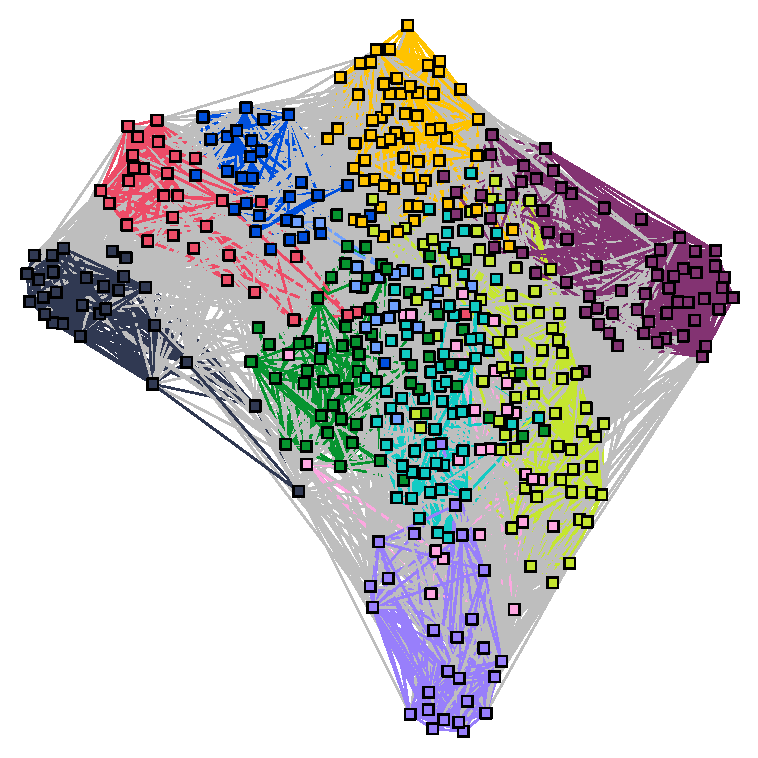
\includegraphics[scale=0.5]{images/stock-network-glasso.eps}
                  \end{figure}
                \end{frame}

                \begin{frame}{Network of stocks via Graphical Lasso}
                  \begin{figure}[!htb]
                    \centering
                    \includegraphics[scale=0.5]{images/augmented-lagrangian.pdf}
                    ~
                    \includegraphics[scale=0.5]{images/primal-residual.pdf}
                  \end{figure}
                \end{frame}

                \begin{frame}{Conclusion}
                  \begin{itemize}
                    \item ADMM is a versatile/flexible optimization framework
                    \item may not be the best for a specific case, but often performs well in practice
                    \item convergence often needs to be proved in a case-by-case scenario
                  \end{itemize}
                \end{frame}

                \section*{Questions?}
\end{document}
